\documentclass[8pt]{article}%
\usepackage{amsfonts}
\usepackage{times}
\usepackage{amsmath}
\usepackage{amssymb}
\usepackage{graphicx}
\usepackage{tikz}
\usepackage[margin=0.2in]{geometry}
\begin{document}
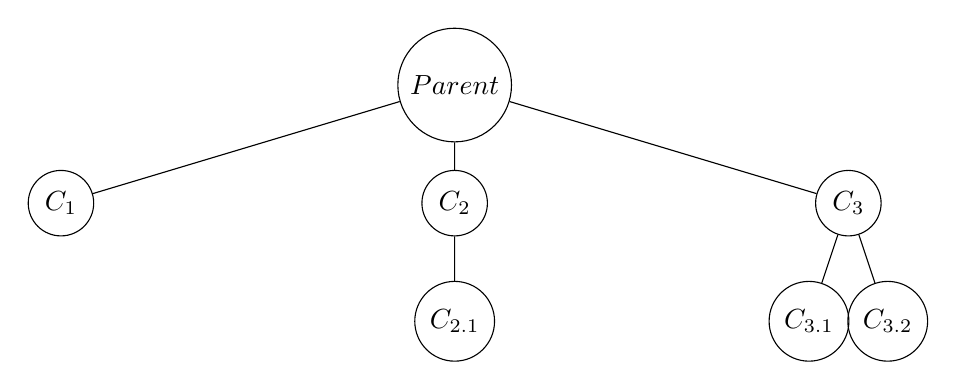
\begin{tikzpicture} [every node/.style={circle,draw}, level 1/.style={sibling distance=50mm},
level 2/.style={sibling distance=10mm},
level 3/.style={sibling distance=15mm}]
[level distance=1.8cm, level 1/.style={sibling distance=3cm},level 2/.style={sibling distance=1.5cm}]
\node {$Parent$}
    child
    {
        node {$C_1$}
    }
    child
    {
        node {$C_2$}
        child
        {
            node {$C_{2.1}$}
        }
    }
    child
    {
        node {$C_3$}
        child
        {
            node {$C_{3.1}$}
        }
        child
        {
            node {$C_{3.2}$}
        }
    };
\end{tikzpicture}
\end{document}
